\documentclass[DIV=15, notitlepage,10pt]{article}
\usepackage{graphicx} % Für die Bilder zum Schwerpunkt
% \usepackage[utf8]{inputenc} % Für Umlaute
\usepackage[german]{babel} 
\usepackage{amsmath}
\usepackage{amssymb}
\usepackage{pgfplots}
\usepackage{subcaption}
\usepackage{titling}

\begin{document}

\title{Projektvorschlag}

\author{
  Jonas Eckhoff
  \and
  Anton Jabs
  \and
  Florian Brach
  \and
  Felix Kieckhäfer
}





\maketitle
Zum Abschluss des Kurses soll ein frei gewähltes Projekt ausgearbeitet und vorgestellt werden. 
Im unserem Abschlussprojekt soll das Auto auf einer unbekannten Strecke fahren und eine Karte der Umgebung erstellen. 
\section{Kreisfahrt}
Im ersten Schritt soll das Auto eine vorgegebene Kreisfahrt absolvieren. Dabei muss das Auto erkennen, dass es sich auf einem Kreis befindet und registrieren, wenn es den Startpunkt wieder erreicht hat. 
Um die Fahrbahn zu erkennen und zu tracken, werden unterschiedliche Markierungen genutzt, zum Beispiel 'Kilometersteine' in regelmäßigen Abständen, klassischen Fahrbahnmarkierungen oder markanten Fixpunkten in der Umgebung. 
Nach Absolvieren der Runde soll das Auto eine Karte erstellen und ggf. an einen verbundenen Computer schicken, um das Ergebnis zu darzustellen. 
Mit der erstellten Karte kann das Auto die Strecke in einem zweiten Durchlauf mit erhöhter Geschwindigkeit durchfahren. 
  
\section{Achtenfahren}
Nach einer erfolgreichen Kreisfahrt soll das Problem durch die Verknüpfung zweier Kreise erschwert werden. Dabei muss das Auto erkennen, dass es nach der ersten Runde noch nicht an der Ausgangsposition angekommen ist, und noch eine zweite Runde fahren muss. \\
Durch die Kreuzung kann das Projekt um die Problemstellung 'Objekterkennung' erweitert werden. Mit Schildern oder aufgeklebten Pfeilen können dem Auto 'Fahrregeln' auferlegt werden, die dann umgesetzt werden müssen. Möglich wäre eine Routenplanung, die über eine Reihe von farbigen Markierungen realisiert wird. 

\begin{figure}[h]
\centering
\begin{minipage}{.5\textwidth}
  \centering
  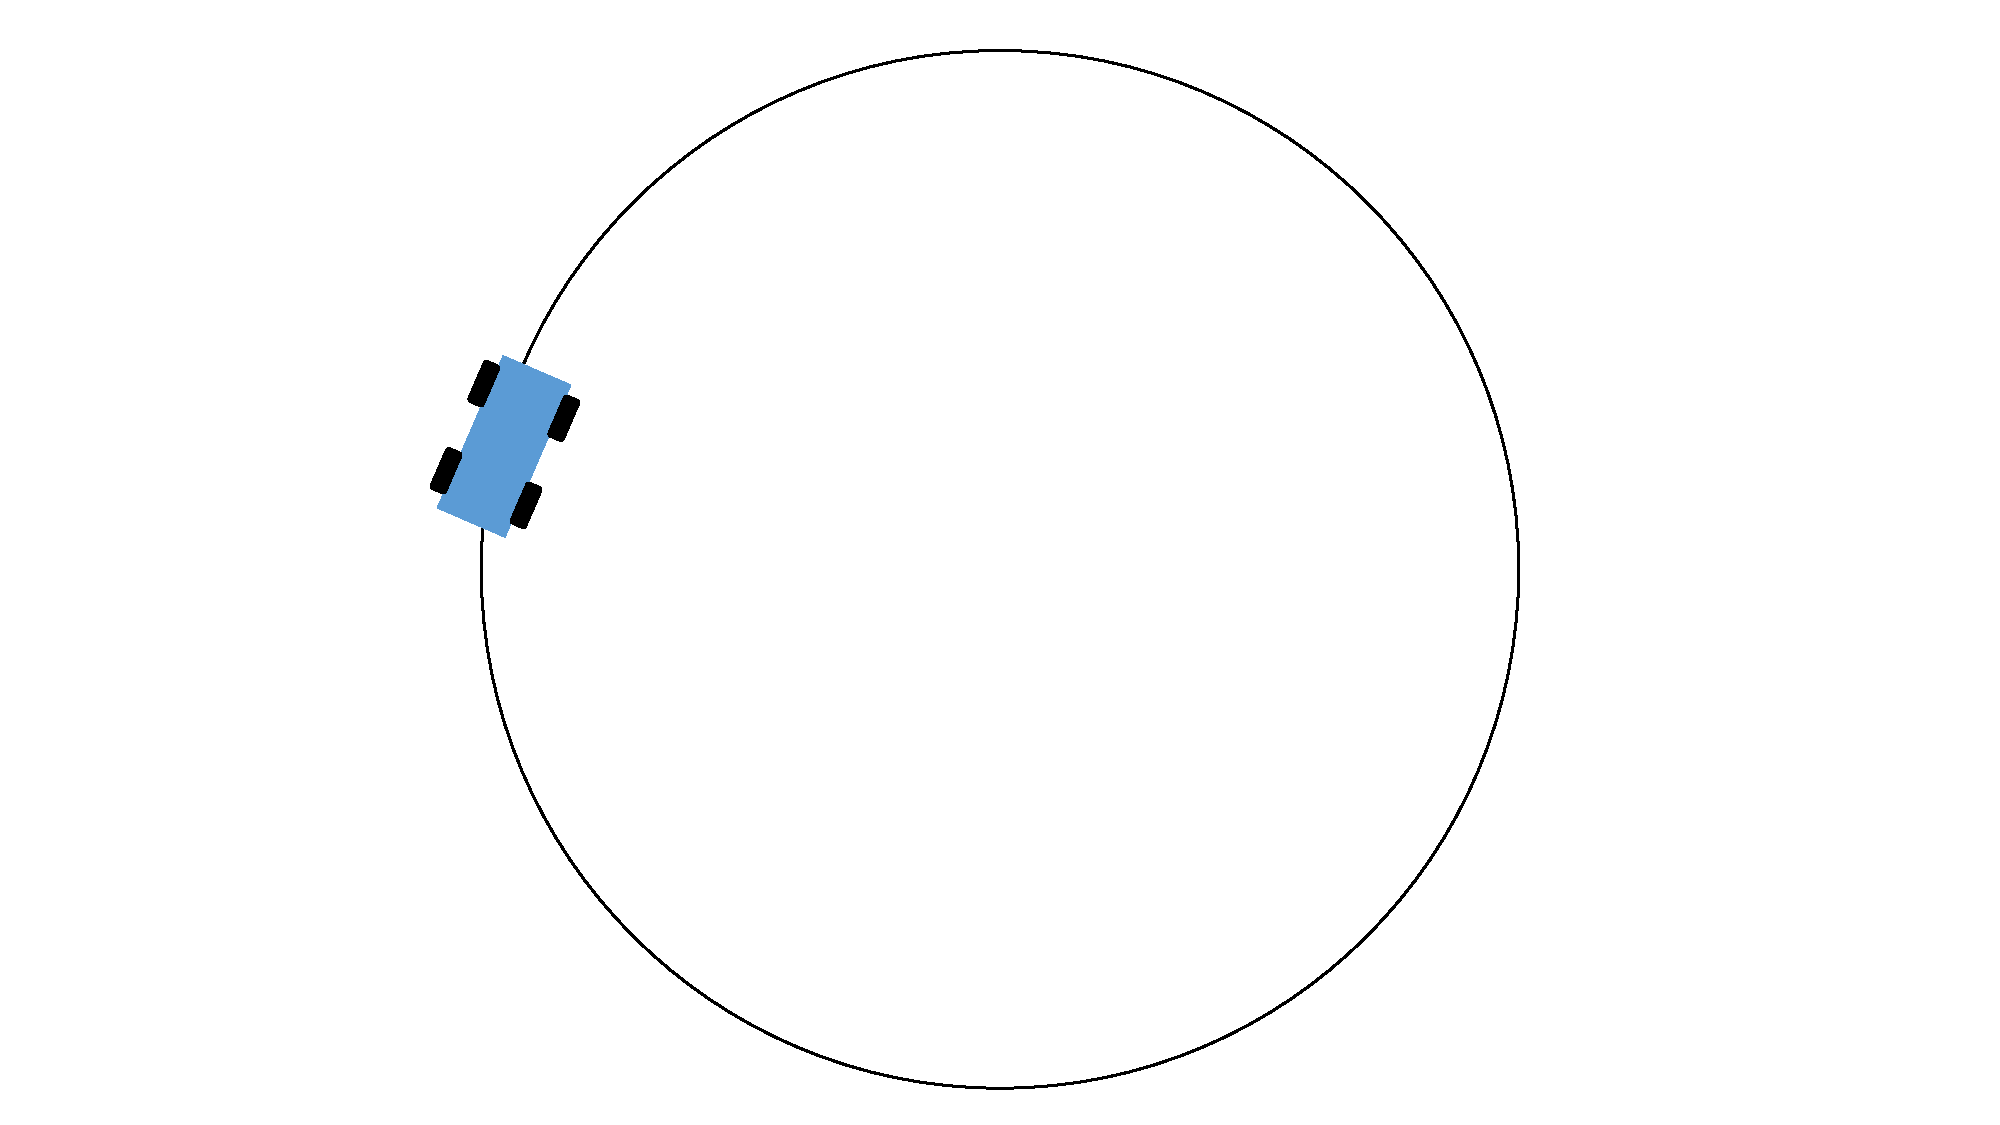
\includegraphics[width=1\linewidth]{Kreis.pdf}
  \captionof{figure}{Kreisfahrt}
  \label{fig:test1}
\end{minipage}%
\begin{minipage}{.5\textwidth}
  \centering
  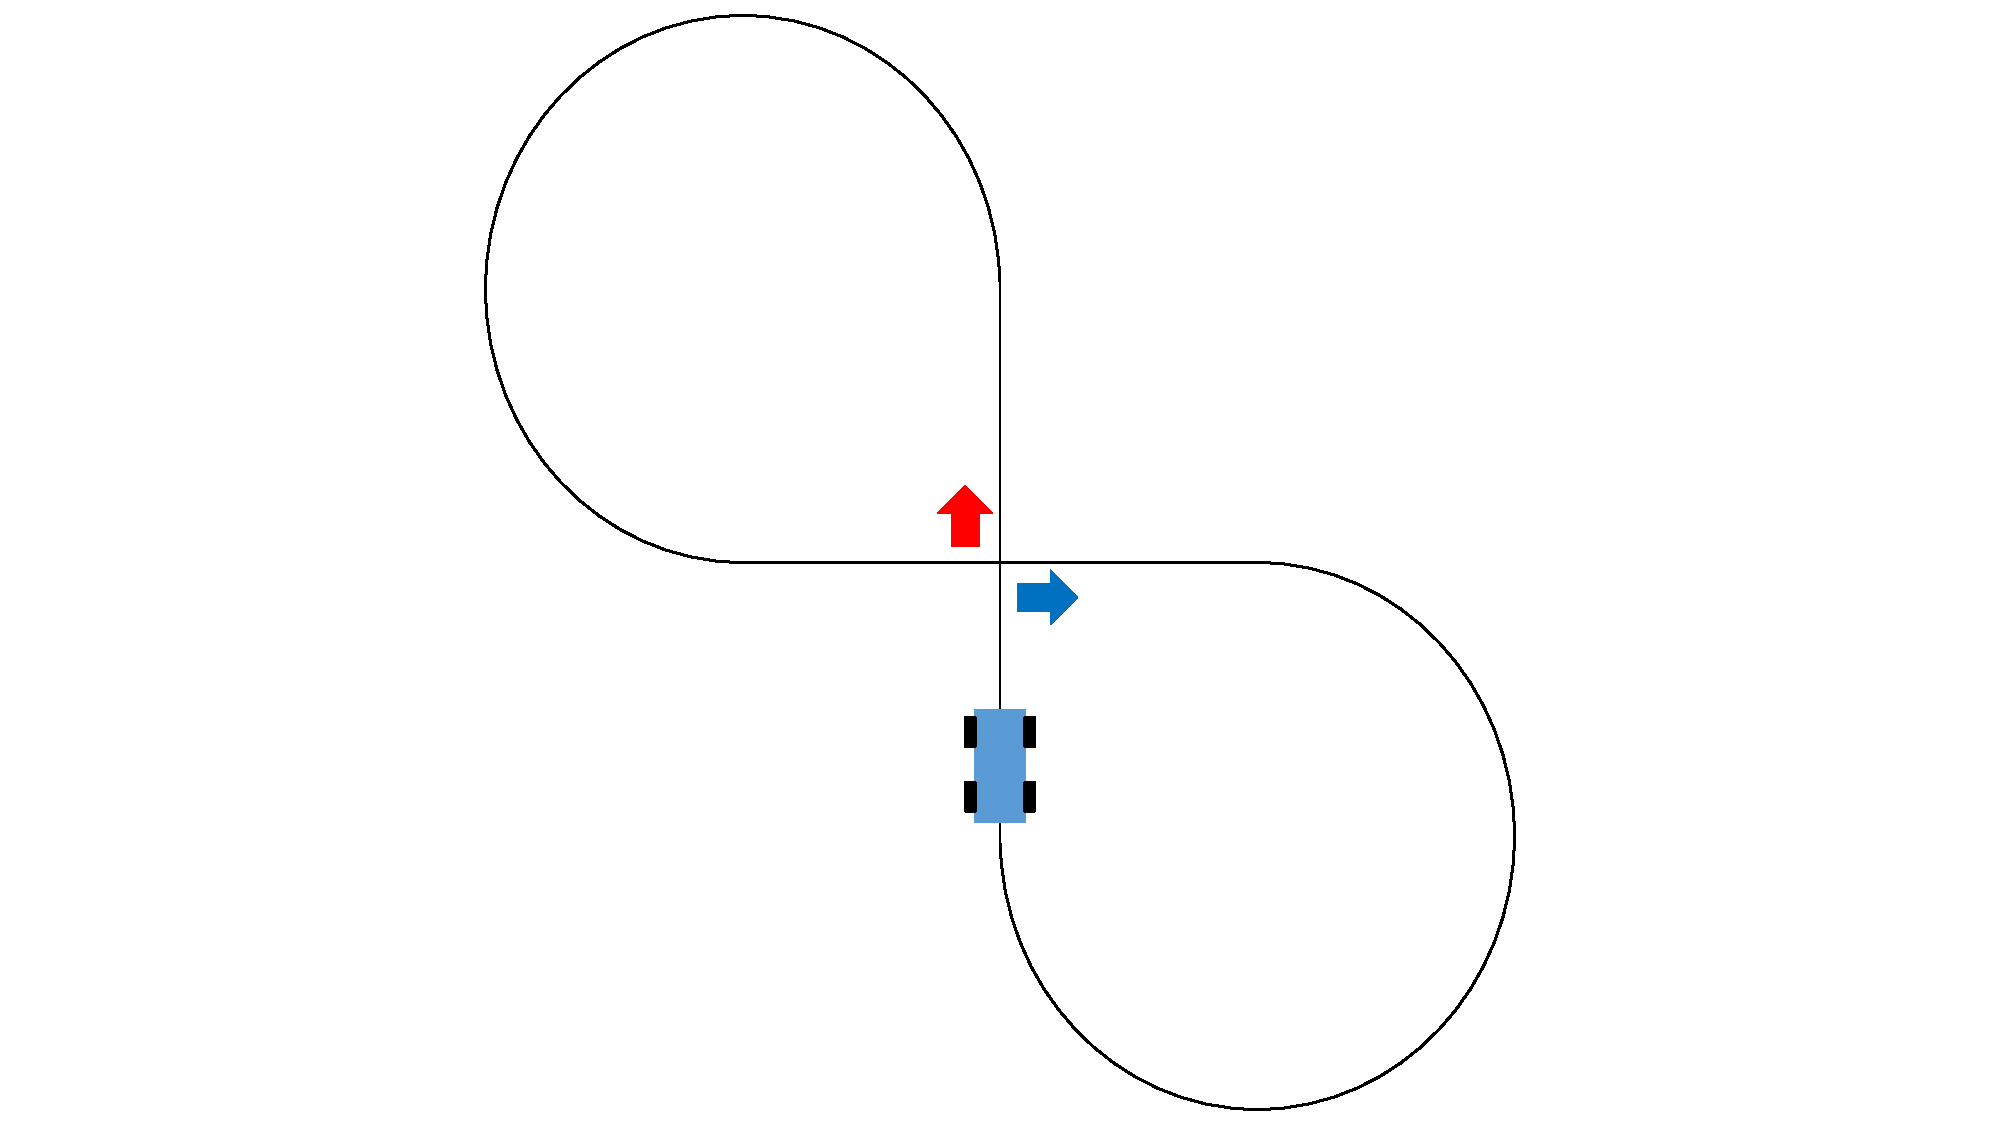
\includegraphics[width=1\linewidth]{Acht2.pdf}
  \captionof{figure}{Achtenfahren}
  \label{fig:test2}
\end{minipage}
\end{figure}

\section{Umsetzung}
Das Projekt kann in mehrere Teilprobleme aufgeteilt werden. Für die Kreisfahrt muss eine Erkennung vorher definierte Markierungen realisiert werden. Darauf aufbauend müssen die Marker abgespeichert und zu einem Pfad zusammengesetzt werden. \\
Für das 'Achtenfahren' muss zusätzlich die Verdrehung des Autos ermittelt werden, um zu gewährleisten, dass das Auto den zweiten Kreis durchfährt. 
Außerdem muss eine Objekterkennung implementiert werden, die es ermöglicht, unterschiedliche farbige Marker zu erkennen und eine entsprechende Fahrroute zu planen. 

\end{document}